\documentclass{report}
\usepackage{times}
\usepackage{epsfig}
\usepackage{alltt}
\usepackage{xspace}
\usepackage{graphicx}
\usepackage{ifpdf}
\usepackage{ifthen}
\usepackage{amsmath}
\usepackage{a4wide}

\graphicspath{{figures/}} 

\ifpdf
\DeclareGraphicsExtensions{.pdf, .jpg, .tif, .png}
\else
\DeclareGraphicsExtensions{.eps, .jpg}
\fi

\newboolean{toseecomment}
\setboolean{toseecomment}{false}
%%change to false to hidde comment 
\newcommand{\comment}[1]{\ifthenelse{\boolean{toseecomment}}{$\blacktriangleright$ \textit{#1}$\blacktriangleleft$}{}}

\newcommand{\commented}[1]{}

\newboolean{seevwspecific}
\setboolean{seevwspecific}{true}
\newcommand{\vwspecific}[1]{\ifthenelse{\boolean{seevwspecific}}{#1}{}}

\newboolean{seecategoryspecific}
\setboolean{seecategoryspecific}{false}
\newcommand{\categoryspecific}[1]{\ifthenelse{\boolean{seecategoryspecific}}{#1}{}}

\newboolean{seestorespecific}
\setboolean{seestorespecific}{true}
\newcommand{\storespecific}[1]{\ifthenelse{\boolean{seestorespecific}}{#1}{}}

\newboolean{seesqueakspecific}
\setboolean{seesqueakspecific}{false}
\newcommand{\squeakspecific}[1]{\ifthenelse{\boolean{seesqueakspecific}}{#1}{}}


\newcommand{\category}[0]
{\ifthenelse{\boolean{seestorespecific}}
	{package\xspace}
	{category\xspace}}

\newcommand{\ct}[1]{\texttt{#1}\xspace}
\newcommand{\stc}[1]{{\small {\sf #1}}\xspace}
\newcommand{\ST}{{\textsc Smalltalk}\xspace}
\newcommand{\tab}{\makebox[4em]{}}
\newcommand{\ttt}[1]{{\tt #1}}
\newcommand{\chev}{\ttt{>>}}
\newcommand{\vw}{VisualWorks\xspace}
\newcommand{\sq}{Squeak\xspace}
\newcommand{\store}{Store\xspace}
\renewcommand{\chaptername}{Exercise}
\newcommand{\exercise}{\vspace{0.2cm}\noindent \textbf{Exercise:}\xspace}

\newsavebox{\fminibox}
\newlength{\fminilength}

% Fait un truc encadre
\newenvironment{fminipage}[1][\linewidth]
  {\setlength{\fminilength}{#1-2\fboxsep-2\fboxrule}
        \begin{lrbox}{\fminibox}\begin{minipage}{\fminilength}}
  { \end{minipage}\end{lrbox}\noindent\fbox{\usebox{\fminibox}}}

% Pareil mais pas encadre (a utiliser pour ne pas couper une fonction

\newenvironment{nminipage}[1][\linewidth]
  {\setlength{\fminilength}{#1}
        \begin{lrbox}{\fminibox}\begin{minipage}{\fminilength}}
  { \end{minipage}\end{lrbox}\noindent\mbox{\usebox{\fminibox}}}

% Un alltt encadre
\newenvironment{falltt}
  {\vspace*{0.3cm}\begin{fminipage}\begin{alltt}}
  {\end{alltt}\end{fminipage}\vspace*{0.3cm}}

% Un alltt pas encadre
\newenvironment{nalltt}
  {\vspace*{0.3cm}\begin{nminipage}\begin{alltt}}
  {\end{alltt}\end{nminipage}\vspace*{0.3cm}}

% Une fonction encadree
\newenvironment{ffonction}[1]
  {\begin{fonction}[#1]
        \begin{fminipage}
\begin{alltt}
\rule{\linewidth}{0.5pt}}
{\end{alltt}\end{fminipage}\end{fonction}}

\newenvironment{codeonepage}
  {\begin{nminipage}\vspace*{0.2cm}\hrule\vspace*{0.1cm}
\begin{alltt}}
  {\end{alltt} \vspace*{-0.2cm}\hrule \vspace*{0.2cm} \end{nminipage}}

\newenvironment{code}
  {\vspace*{0.1cm}\hrule\vspace*{-0.1cm}\begin{alltt}}
  {\end{alltt}\vspace*{-0.2cm}\hrule \vspace*{0.1cm}}


%%% for separate compilation
\let\wholebook=\relax

\begin{document}
\title{Smalltalk Exercises}
\author{
Prof. Dr. Roel Wuyts\\
{\small Universit\'{e} Libre de Bruxelles} \\
{\small Bruxelles, Belgique} \\
{\small {\tt \{roel.wuyts\}@ulb.ac.be}}\\
{\small {\tt http://www.ulb.ac.be/di/rwuyts/AnCo$\_$0405/}}
}

\maketitle

\setboolean{seevwspecific}{true}
\setboolean{seesqspecific}{false}
\setboolean{seecategoryspecific}{false}
\setboolean{seeparcelspecific}{true}
\setboolean{seestorespecific}{false}
\setboolean{seesqueaksourcespecific}{false}
\setboolean{seesqueakspecific}{false}

\ifx\wholebook\relax\else
\documentclass{report}
\usepackage{times}
\usepackage{epsfig}
\usepackage{alltt}
\usepackage{xspace}
\usepackage{graphicx}
\usepackage{ifpdf}
\usepackage{ifthen}
\usepackage{amsmath}
\usepackage{a4wide}

\graphicspath{{figures/}} 

\ifpdf
\DeclareGraphicsExtensions{.pdf, .jpg, .tif, .png}
\else
\DeclareGraphicsExtensions{.eps, .jpg}
\fi

\newboolean{toseecomment}
\setboolean{toseecomment}{false}
%%change to false to hidde comment 
\newcommand{\comment}[1]{\ifthenelse{\boolean{toseecomment}}{$\blacktriangleright$ \textit{#1}$\blacktriangleleft$}{}}

\newcommand{\commented}[1]{}

\newboolean{seevwspecific}
\setboolean{seevwspecific}{true}
\newcommand{\vwspecific}[1]{\ifthenelse{\boolean{seevwspecific}}{#1}{}}

\newboolean{seecategoryspecific}
\setboolean{seecategoryspecific}{false}
\newcommand{\categoryspecific}[1]{\ifthenelse{\boolean{seecategoryspecific}}{#1}{}}

\newboolean{seestorespecific}
\setboolean{seestorespecific}{true}
\newcommand{\storespecific}[1]{\ifthenelse{\boolean{seestorespecific}}{#1}{}}

\newboolean{seesqueakspecific}
\setboolean{seesqueakspecific}{false}
\newcommand{\squeakspecific}[1]{\ifthenelse{\boolean{seesqueakspecific}}{#1}{}}


\newcommand{\category}[0]
{\ifthenelse{\boolean{seestorespecific}}
	{package\xspace}
	{category\xspace}}

\newcommand{\ct}[1]{\texttt{#1}\xspace}
\newcommand{\stc}[1]{{\small {\sf #1}}\xspace}
\newcommand{\ST}{{\textsc Smalltalk}\xspace}
\newcommand{\tab}{\makebox[4em]{}}
\newcommand{\ttt}[1]{{\tt #1}}
\newcommand{\chev}{\ttt{>>}}
\newcommand{\vw}{VisualWorks\xspace}
\newcommand{\sq}{Squeak\xspace}
\newcommand{\store}{Store\xspace}
\renewcommand{\chaptername}{Exercise}
\newcommand{\exercise}{\vspace{0.2cm}\noindent \textbf{Exercise:}\xspace}

\newsavebox{\fminibox}
\newlength{\fminilength}

% Fait un truc encadre
\newenvironment{fminipage}[1][\linewidth]
  {\setlength{\fminilength}{#1-2\fboxsep-2\fboxrule}
        \begin{lrbox}{\fminibox}\begin{minipage}{\fminilength}}
  { \end{minipage}\end{lrbox}\noindent\fbox{\usebox{\fminibox}}}

% Pareil mais pas encadre (a utiliser pour ne pas couper une fonction

\newenvironment{nminipage}[1][\linewidth]
  {\setlength{\fminilength}{#1}
        \begin{lrbox}{\fminibox}\begin{minipage}{\fminilength}}
  { \end{minipage}\end{lrbox}\noindent\mbox{\usebox{\fminibox}}}

% Un alltt encadre
\newenvironment{falltt}
  {\vspace*{0.3cm}\begin{fminipage}\begin{alltt}}
  {\end{alltt}\end{fminipage}\vspace*{0.3cm}}

% Un alltt pas encadre
\newenvironment{nalltt}
  {\vspace*{0.3cm}\begin{nminipage}\begin{alltt}}
  {\end{alltt}\end{nminipage}\vspace*{0.3cm}}

% Une fonction encadree
\newenvironment{ffonction}[1]
  {\begin{fonction}[#1]
        \begin{fminipage}
\begin{alltt}
\rule{\linewidth}{0.5pt}}
{\end{alltt}\end{fminipage}\end{fonction}}

\newenvironment{codeonepage}
  {\begin{nminipage}\vspace*{0.2cm}\hrule\vspace*{0.1cm}
\begin{alltt}}
  {\end{alltt} \vspace*{-0.2cm}\hrule \vspace*{0.2cm} \end{nminipage}}

\newenvironment{code}
  {\vspace*{0.1cm}\hrule\vspace*{-0.1cm}\begin{alltt}}
  {\end{alltt}\vspace*{-0.2cm}\hrule \vspace*{0.1cm}}



\begin{document}
\fi

\chapter{Basics of the VisualWorks Smalltalk Environment}

\section{Starting up}
Smalltalk is an interpreted language: the source code is translated 
to Smalltalk-byte codes, which is then interpreted and executed by 
the Smalltalk Virtual Machine. (Note that this is an approximation 
because Smalltalk dialects were also the first languages to develop 
Just in Time compilation, i.e. a method is compiled into byte-codes 
but also into native code that is directly called instead of  
interpreting the byte codes.)

When looking at VisualWorks Smalltalk, there are three important 
files:

\begin{description}
\item{visual.sou}  (ASCII): contains the textual code of the initial 
classes of the system. 
\item{visual.im} (Binary): contains byte code of all the object of the 
system, the libraries and the modifications you made.
\item{visual.cha} (ASCII): contains all the modifications made in the 
image-file since this was created.
\end{description}

On MacIntosh, to open an image:
\begin{itemize}
\item Drag the file 'visual.im' on the virtual machine to start the image.
\item If  you want to start your own image, just double click on it or 
drag it over the virtual machine.
\end{itemize}

On Solaris: you should invoke the virtual machine passing it an image 
as parameter. For the first opening, execute the first script that per default 
uses the original image the script is installation dependent but 
should look like path/bin/visualworks path/image/visual.im
Then after you can specify your own image. 

After opening the image, and thus starting a Smalltalk session, you 
see two windows : the VisualWorks launcher (with menu, buttons and a 
transcript), and a Workspace window (the one containing text). You 
can minimize or close this last one, since we do not need it for the 
moment.

The launcher is the starting point for working with your environment 
and for the opening of all the programming tools that you might need. 
To begin, we will first create a fresh image.

\paragraph{Creating a fresh image.}
We are going to create a new image for this lesson. 
\begin{itemize}
\item	select �Save As...� in the file-menu
\item	when the system prompts you for the name for the new image, you 
type lesson.
\item	the image is saved in the image directory 
\item	Have a look at the Transcript, and note what it says
\end{itemize}

The \stc{Transcript} is the lower part of the Launcher, and gives you 
system messages, like the one you see right now. We will see later on 
how you can put your own messages there.

\paragraph{About the mouse.}
VisualWorks (or rather the older precedent) was the first application 
to use multiple overlapping windows and a mouse. It extensively uses 
three mouse buttons, that are context sensitive and can be used 
everywhere throughout Smalltalk:
\begin{itemize}
\item	the left mouse button is the select button
\item	the middle button is the operate button
\item	the right button is the window button
\end{itemize}

On a Macintosh, where only one button is available, you have to use 
some keyboard keys together with pressing your mouse button:
\begin{itemize}
\item	the select button is the one button itself
\item	for the operate button, press the button while holding the alt-key 
pressed
\item	for the window button, press the button while holding the apple-key 
pressed
\end{itemize}

\section{Selecting text, and doing basic text manipulations}
One of the basic manipulations you do when programming is working 
with text. Therefore, this section introduces you to the different 
ways you can select text, and manipulate these selections.

The basic way of selecting text is by clicking in front of the first 
character you want to select, and dragging your mouse to the last 
character you want in the selection while keeping the button pressed 
down. Selected text will be highlighted. 

\exercise Select some parts of text in the Transcript.
You can also select a single word by double clicking on it. When the 
text is delimited by '' (single quotes), "" (double quotes), () 
(parentheses), [] (brackets), or {} (braces), you can select anything 
in between by double clicking just after the first delimiter.

\exercise Try these new selection techniques.


Now have a look at the text operations. Select a piece of text in the 
\stc{Transcript}, and bring on the operate menu. Note that you have to 
keep your mouse button pressed to keep seeing the window. 

\exercise Copy this piece of text, and paste it after your 
selection. Afterwards cut the newly inserted piece of text.

\exercise See if there is an occurrence of the word visual in the 
Transcript. Note that to find things in a text window, there is no 
need to select text. Just bring up the operate menu . 

\exercise Replace the word visual with C++ using the replace 
operation (if it does not contain Smalltalk, add this word or replace 
something else). Take your time and explore the different options of 
the replace operation.

\exercise Bring up the operate menu, but don't select anything yet. 
Press and hold the shift button, and select paste in the operation 
menu. What happens ?

\section{Opening a WorkSpace Window}
We will now open a workspace window, a text window much like the 
Transcript, you use to type text and expressions and evaluate them. 
To open a workspace:
\begin{itemize}
\item	select the tools menu in the Launcher
\item	from the tools menu, select Workspace
\item	You will see a framing rectangle (with your mouse in the upper left 
corner), that indicates the position where the Workspace will open. 
Before you click, you can move your mouse around to change this 
position. Click one time once you have found a good spot for your 
Workspace. 

\item	Now your mouse is in the bottom right corner, and you can adjust 
the size. If you click once more, once you have given it the size you 
like, the Workspace window appears.
\end{itemize}

This is the basic way of opening any kind of VisualWorks application 
windows. Experiment with it until you feel comfortable with it.

\paragraph{The Window menu.}
To resize a window on the Macintosh, click in the lower right corner 
while holding the alt-button. On a PC or Sun, you resize VisualWorks 
windows the same way as any other window.

Once you have opened your Workspace window, bring up the window menu, 
and experiment with it. Note that this menu is the same for each 
window, and contains the very basic window manipulations. 

\section{Evaluating Expressions}
In the Workspace, type : 3.
Select it, and bring up the operate menu.
In the operate you will see the next three different options for 
evaluating text and getting the result:

\begin{description}
\item[do it:] do it evaluates the current selection, and does not show any 
result of the evaluation result. 
\item[print it:] prints the result of the evaluation after your selection. 
The result is automatically highlighted, so you can easily delete it 
if you want to.
\item[inspect it:] opens an inspector on the result of the evaluation.
\end{description}

The distinction before these three operations is essential, so check 
that you REALLY understand their differences
\exercise Select 3, bring up the operate menu, and select print it.

\exercise Print the result of 3+4
\exercise Type \stc{Date today} and print it. Afterwards, select it again 
and inspect it.

After exercise 9, you will have an inspector on the result of the 
evaluation of the expression Date today (this tells VisualWorks to 
create an object containing the current date). This Inspector Window 
consists of two parts: the left one is a list view containing self (a 
pseudo variable containing the object you are inspecting) and the 
instance variables of the object. Right is a text field.

\exercise Click on \stc{self} in the inspector. What do you get ? Does 
it resemble the result shown by printstring ?

\exercise Select day. What do you get ? Now change this value, 
bring up the operate menu, and select accept it. Click again on 
\stc{self}. 
Any difference? 

\exercise In the inspector edit field, type the following: self 
weekday, select it and print it. This causes the message weekday to 
be sent to self (i.e. the date object), and the result is printed. 
Experiment with other expressions like:
\begin{code}
self daysInMonth
self monthName
\end{code}

Close the inspector when you are finished.
\exercise	Type in the Workspace the following expression: Time 
now, and inspect it. Have a look at self and the instance variables.

\exercise Type in the Workspace the following expression: \stc{Time 
dateAndTimeNow}. This tells VisualWorks to create an object 
representing both today's date and the current time, and open an 
inspector on it. Select the item \stc{self} in the inspector. [Note that 
self is an object called an Array. It holds on to two other objects 
(elements 1 and 2). You can inspect each element to get either the 
time or the date object.

\paragraph{Using the System Transcript.} 
We have already seen that the Transcript is a text window at the 
bottom of the Launcher where the system informs you important 
information. You can also use the Transcript yourself as a very cheap 
user interface.

If you have a Workspace open, place it so that it does not cover the 
System Transcript. Otherwise, open one and take care of  where you 
put it. Now, in the Workspace, type:
\begin{code}
	Transcript cr.
	Transcript show: 'This is a test'.
	Trancript cr.
\end{code}

Select these 3 lines and evaluate (do It) them with do it.
This will cause the string This is a test to be printed in the 
Transcript, preceeded and followed by a carriage return. Note that 
the argument of the show: message was a literal string (you see this 
because it is contained in single quotes). It is important to know, 
because the argument of the show: method always has to be a string. 
This means that if you want any non-string object to be printed (like 
a Number for example), you first have to convert it to a string by 
sending the message printString to it. For example, type in the 
workspace the following expression and evaluate it:

	\stc{Transcript show: 42 printString, 'is the answer to the Universe'}
Note here that the comma is used to concatenate the two strings that 
are passed to the show: message 42 printString and 'is the answer to 
the Universe'.

\exercise Experiment on your own with different expressions.
	\stc{Transcript cr ; show: �This is a test� ; cr}
Explain why this expression gives the same result that before. What 
is the semantics of  �;� ?



\ifx\wholebook\relax\else\end{document}\fi

\ifx\wholebook\relax\else
\documentclass{report}
\usepackage{times}
\usepackage{epsfig}
\usepackage{alltt}
\usepackage{xspace}
\usepackage{graphicx}
\usepackage{ifpdf}
\usepackage{ifthen}
\usepackage{amsmath}
\usepackage{a4wide}

\graphicspath{{figures/}} 

\ifpdf
\DeclareGraphicsExtensions{.pdf, .jpg, .tif, .png}
\else
\DeclareGraphicsExtensions{.eps, .jpg}
\fi

\newboolean{toseecomment}
\setboolean{toseecomment}{false}
%%change to false to hidde comment 
\newcommand{\comment}[1]{\ifthenelse{\boolean{toseecomment}}{$\blacktriangleright$ \textit{#1}$\blacktriangleleft$}{}}

\newcommand{\commented}[1]{}

\newboolean{seevwspecific}
\setboolean{seevwspecific}{true}
\newcommand{\vwspecific}[1]{\ifthenelse{\boolean{seevwspecific}}{#1}{}}

\newboolean{seecategoryspecific}
\setboolean{seecategoryspecific}{false}
\newcommand{\categoryspecific}[1]{\ifthenelse{\boolean{seecategoryspecific}}{#1}{}}

\newboolean{seestorespecific}
\setboolean{seestorespecific}{true}
\newcommand{\storespecific}[1]{\ifthenelse{\boolean{seestorespecific}}{#1}{}}

\newboolean{seesqueakspecific}
\setboolean{seesqueakspecific}{false}
\newcommand{\squeakspecific}[1]{\ifthenelse{\boolean{seesqueakspecific}}{#1}{}}


\newcommand{\category}[0]
{\ifthenelse{\boolean{seestorespecific}}
	{package\xspace}
	{category\xspace}}

\newcommand{\ct}[1]{\texttt{#1}\xspace}
\newcommand{\stc}[1]{{\small {\sf #1}}\xspace}
\newcommand{\ST}{{\textsc Smalltalk}\xspace}
\newcommand{\tab}{\makebox[4em]{}}
\newcommand{\ttt}[1]{{\tt #1}}
\newcommand{\chev}{\ttt{>>}}
\newcommand{\vw}{VisualWorks\xspace}
\newcommand{\sq}{Squeak\xspace}
\newcommand{\store}{Store\xspace}
\renewcommand{\chaptername}{Exercise}
\newcommand{\exercise}{\vspace{0.2cm}\noindent \textbf{Exercise:}\xspace}

\newsavebox{\fminibox}
\newlength{\fminilength}

% Fait un truc encadre
\newenvironment{fminipage}[1][\linewidth]
  {\setlength{\fminilength}{#1-2\fboxsep-2\fboxrule}
        \begin{lrbox}{\fminibox}\begin{minipage}{\fminilength}}
  { \end{minipage}\end{lrbox}\noindent\fbox{\usebox{\fminibox}}}

% Pareil mais pas encadre (a utiliser pour ne pas couper une fonction

\newenvironment{nminipage}[1][\linewidth]
  {\setlength{\fminilength}{#1}
        \begin{lrbox}{\fminibox}\begin{minipage}{\fminilength}}
  { \end{minipage}\end{lrbox}\noindent\mbox{\usebox{\fminibox}}}

% Un alltt encadre
\newenvironment{falltt}
  {\vspace*{0.3cm}\begin{fminipage}\begin{alltt}}
  {\end{alltt}\end{fminipage}\vspace*{0.3cm}}

% Un alltt pas encadre
\newenvironment{nalltt}
  {\vspace*{0.3cm}\begin{nminipage}\begin{alltt}}
  {\end{alltt}\end{nminipage}\vspace*{0.3cm}}

% Une fonction encadree
\newenvironment{ffonction}[1]
  {\begin{fonction}[#1]
        \begin{fminipage}
\begin{alltt}
\rule{\linewidth}{0.5pt}}
{\end{alltt}\end{fminipage}\end{fonction}}

\newenvironment{codeonepage}
  {\begin{nminipage}\vspace*{0.2cm}\hrule\vspace*{0.1cm}
\begin{alltt}}
  {\end{alltt} \vspace*{-0.2cm}\hrule \vspace*{0.2cm} \end{nminipage}}

\newenvironment{code}
  {\vspace*{0.1cm}\hrule\vspace*{-0.1cm}\begin{alltt}}
  {\end{alltt}\vspace*{-0.2cm}\hrule \vspace*{0.1cm}}


\begin{document}
\fi


\chapter{Objects and expressions}

This lesson is about reading and understanding Smalltalk
expressions, and differentiating between different types of
messages and receivers. Note that in the expressions you will be
asked to read and evaluate, you can assume that the implementation
of methods generally corresponds to what their message names imply
(i.e. 2 + 2 = 4). \\
\exercise For each of the Smalltalk
expressions below, fill in the answers:

\begin{code}
3 + 4
\end{code}
\begin{itemize}
\item What is the receiver object?
\item What is the message selector?
\item What is/are the argument (s)?
\item What is the message?
\item What is the result returned by evaluating this expression?
\end{itemize}

\begin{code}
Date today
\end{code}
\begin{itemize}
\item What is the receiver object?
\item What is the message selector?
\item What is/are the argument (s)?
\item What is the message?
\item What is the result returned by evaluating this expression?
\end{itemize}

\begin{code}
anArray at: 1 put: 'hello'
\end{code}

\begin{itemize}
\item What is the receiver object?
\item What is the message selector?
\item What is/are the argument (s)?
\item What is the message?
\item What is the result returned by evaluating this expression?
\end{itemize}

\exercise What kind of object does the literal expression \stc{'Hello, Dave'} describe?

\exercise What kind of object does the literal expression \stc{\#Node1} describe?

\exercise What kind of object does the literal expression \stc{\#(1 2 3)} describe?

\exercise What can one assume about a variable named \stc{Transcript}?

\exercise What can one assume about a variable named \stc{rectangle}?

\exercise Examine the following expression:

\begin{code}
\ttt{|} anArray \ttt{|}
anArray := #('first' 'second' 'third' 'fourth').
^anArray at: 2
\end{code}

What is the resulting value when it is evaluated (\^{ } means return)?
What happens if you remove the \^{ }. Explain

\exercise Which sets of parentheses are redundant with regard to
evaluation of the following expressions:

\begin{code}
((3 + 4) + (2 * 2) + (2 * 3))

(x isZero)
   ifTrue: [....]
(x includes: y)
   ifTrue: [....]
\end{code}

\exercise Guess what are the results of the following expressions

\begin{code}
6 + 4 / 2
1 + 3 negated
1 + (3 negated)
2 raisedTo: 3 + 2
2 negated raisedTo: 3 + 2
\end{code}

\exercise Examine the following expression:
\begin{code}
25@50
\end{code}
\begin{itemize}
\item What is the receiver object?
\item What is the message selector?
\item What is/are the argument (s)?
\item What is the message?
\item What is the result returned by evaluating this expression?
\end{itemize}

\exercise Examine the following expression and write down the sequence of steps that the Smalltalk system would take to execute the following expression:
\begin{code}
Date today daysInMonth
\end{code}
\exercise Examine the following expression and write down the
sequence of steps that the Smalltalk system would take to execute
the following expression:
\begin{code}
Transcript show: (45 + 9) printString
\end{code}
\exercise Examine the following expression and write down the
sequence of steps that the Smalltalk system would take to execute
the following expression:
\begin{code}
5@5 extent: 6.0 truncated @ 7
\end{code}
\exercise During lecture, we saw how to write strings to the
Transcript, and how the message \texttt{printString} could be sent
to any non-string object to obtain a string representation. Now
write a Smalltalk expression to print the result of \texttt{34 +
89} on the Transcript. Test your code !

\newpage
\exercise Examine the block expression:

\begin{code}
\ttt{|} anArray sum \ttt{|}
sum := 0.
anArray := #(21 23 53 66 87).
anArray do: [:item | sum := sum + item].
sum
\end{code}

What is the final result of sum ? How could this piece of code be
rewritten to use explicit array indexing (with the method
\texttt{at:} ) to access the array elements\footnote{Note this is
how you would proceed with Java or C++}? Test your version.
Rewrite this code using inject:into:


\ifx\wholebook\relax\else\end{document}\fi

\ifx\wholebook\relax\else
\documentclass{report}
\usepackage{times}
\usepackage{epsfig}
\usepackage{alltt}
\usepackage{xspace}
\usepackage{graphicx}
\usepackage{ifpdf}
\usepackage{ifthen}
\usepackage{amsmath}
\usepackage{a4wide}

\graphicspath{{figures/}} 

\ifpdf
\DeclareGraphicsExtensions{.pdf, .jpg, .tif, .png}
\else
\DeclareGraphicsExtensions{.eps, .jpg}
\fi

\newboolean{toseecomment}
\setboolean{toseecomment}{false}
%%change to false to hidde comment 
\newcommand{\comment}[1]{\ifthenelse{\boolean{toseecomment}}{$\blacktriangleright$ \textit{#1}$\blacktriangleleft$}{}}

\newcommand{\commented}[1]{}

\newboolean{seevwspecific}
\setboolean{seevwspecific}{true}
\newcommand{\vwspecific}[1]{\ifthenelse{\boolean{seevwspecific}}{#1}{}}

\newboolean{seecategoryspecific}
\setboolean{seecategoryspecific}{false}
\newcommand{\categoryspecific}[1]{\ifthenelse{\boolean{seecategoryspecific}}{#1}{}}

\newboolean{seestorespecific}
\setboolean{seestorespecific}{true}
\newcommand{\storespecific}[1]{\ifthenelse{\boolean{seestorespecific}}{#1}{}}

\newboolean{seesqueakspecific}
\setboolean{seesqueakspecific}{false}
\newcommand{\squeakspecific}[1]{\ifthenelse{\boolean{seesqueakspecific}}{#1}{}}


\newcommand{\category}[0]
{\ifthenelse{\boolean{seestorespecific}}
	{package\xspace}
	{category\xspace}}

\newcommand{\ct}[1]{\texttt{#1}\xspace}
\newcommand{\stc}[1]{{\small {\sf #1}}\xspace}
\newcommand{\ST}{{\textsc Smalltalk}\xspace}
\newcommand{\tab}{\makebox[4em]{}}
\newcommand{\ttt}[1]{{\tt #1}}
\newcommand{\chev}{\ttt{>>}}
\newcommand{\vw}{VisualWorks\xspace}
\newcommand{\sq}{Squeak\xspace}
\newcommand{\store}{Store\xspace}
\renewcommand{\chaptername}{Exercise}
\newcommand{\exercise}{\vspace{0.2cm}\noindent \textbf{Exercise:}\xspace}

\newsavebox{\fminibox}
\newlength{\fminilength}

% Fait un truc encadre
\newenvironment{fminipage}[1][\linewidth]
  {\setlength{\fminilength}{#1-2\fboxsep-2\fboxrule}
        \begin{lrbox}{\fminibox}\begin{minipage}{\fminilength}}
  { \end{minipage}\end{lrbox}\noindent\fbox{\usebox{\fminibox}}}

% Pareil mais pas encadre (a utiliser pour ne pas couper une fonction

\newenvironment{nminipage}[1][\linewidth]
  {\setlength{\fminilength}{#1}
        \begin{lrbox}{\fminibox}\begin{minipage}{\fminilength}}
  { \end{minipage}\end{lrbox}\noindent\mbox{\usebox{\fminibox}}}

% Un alltt encadre
\newenvironment{falltt}
  {\vspace*{0.3cm}\begin{fminipage}\begin{alltt}}
  {\end{alltt}\end{fminipage}\vspace*{0.3cm}}

% Un alltt pas encadre
\newenvironment{nalltt}
  {\vspace*{0.3cm}\begin{nminipage}\begin{alltt}}
  {\end{alltt}\end{nminipage}\vspace*{0.3cm}}

% Une fonction encadree
\newenvironment{ffonction}[1]
  {\begin{fonction}[#1]
        \begin{fminipage}
\begin{alltt}
\rule{\linewidth}{0.5pt}}
{\end{alltt}\end{fminipage}\end{fonction}}

\newenvironment{codeonepage}
  {\begin{nminipage}\vspace*{0.2cm}\hrule\vspace*{0.1cm}
\begin{alltt}}
  {\end{alltt} \vspace*{-0.2cm}\hrule \vspace*{0.2cm} \end{nminipage}}

\newenvironment{code}
  {\vspace*{0.1cm}\hrule\vspace*{-0.1cm}\begin{alltt}}
  {\end{alltt}\vspace*{-0.2cm}\hrule \vspace*{0.1cm}}



\begin{document}
\fi

\chapter{Counter Example}
This document provides the initial exercise you should do to be
familiar with Smalltalk syntax and VisualWorks 7.


\section*{A Simple Counter}
We want you to implement a simple counter that follows the small example given
below. Please note that we will ask you to define a test for this example.

\begin{code}
|counter|
counter := SimpleCounter new.
counter increment; increment.
counter decrement.
counter value = 1
\end{code}


\section*{Creating your own class}
In this part you will create the first class. In traditional Smalltalk environments a class is associated with a category (a folder containing the classes of your project). 

\storespecific{When we are using \store, categories are replaced by package. 
Therefore in \vw with \store you define a package and define your class within this package.}
The steps we will do are the same ones every  time you create a class, so memorize them well. We are going to create a class \texttt{SimpleCounter} in a \category called \texttt{DemoCounter}. Note that are you will be all versioning your code in the \store database your package have to have a different name. So prefix them with your initials.

\storespecific{
\subsection*{Creating a Package}
In the System Browser, click on \texttt{Local Image} (left button
of the mouse) and select \texttt{New}$>>$\texttt{Package}. The
system will ask you a name. You should write \texttt{DemoCounter}.
This new package will be created and added to the list.}

\squeakspecific{
\subsection*{Creating a Class category}
In the System Browser, click on the left pane and select add. The
system will ask you a name. You should write \texttt{DemoCounter}.
This new \category will be created and added to the list.}

\vwspecific{\subsection*{With Namespace}
In \vw you can also define your own namespace. If you do so you will have to define your namespace then define the class in this namespace. For now we suggest you to use the default namespace called \ct{Smalltalk}.}

\subsection*{Creating a Class}


\storespecific{
\begin{figure}[htbp]
\begin{center}
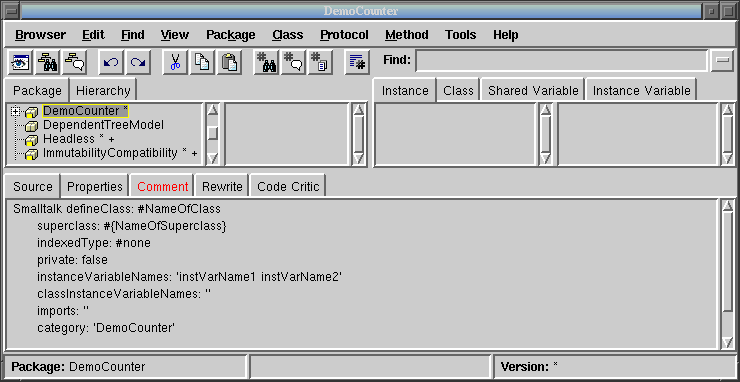
\includegraphics[scale=0.5]{nlesson3Fig4Package}
\caption{Your package is created.}
\end{center}
\end{figure}}

\categoryspecific{
\begin{figure}[htbp]
\begin{center}
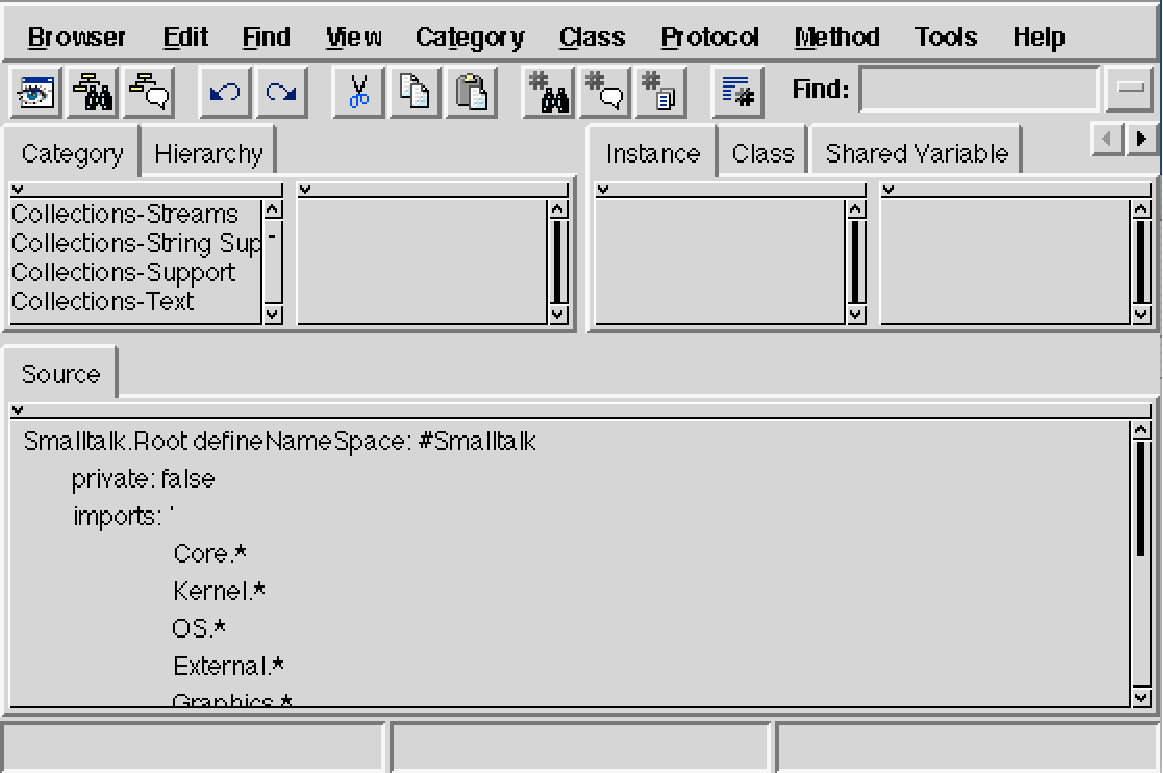
\includegraphics[scale=0.5]{nlesson3Fig4CategoryVW}
\caption{Your category is created.}
\end{center}
\end{figure}}

Creating a class requires five steps. They consist basically of
editing the class definition template to specify the class you
want to create. \storespecific{\textit{Before you begin, make sure that only the package \texttt{DemoCounter} is selected.}}

\begin{enumerate}
\item \textbf{Superclass Specification}. First, you should replace
the word \texttt{NameOfSuperclass} with the word \texttt{\vwspecific{Core.}Object}\vwspecific{\footnote{We will see when we will be building a user interface for this object that we will change its superclass}}. Thus, you specify the superclass of the class you are
creating. 

\item \textbf{Class Name}. Next, you should fill in the name of
your class by replacing the word \texttt{NameOfClass} with the
word \texttt{SimpleCounter}. Take care that the name of the class
starts with a capital letter and that you do not remove the \#
sign in front of \texttt{NameOfClass}.

\item \textbf{Instance Variable Specification}. Then, you should
fill in the names of the instance variables of this class. We need
one instance variable called \texttt{value}. You add it by
replacing the words \textit{instVarName1} and
\textit{instVarName2} with the word \texttt{value}.Take
care that you leave the string quotes!

\item \textbf{Class Variable Specification}. As we do not need any class variable make sure that the argument  for the class instance variables is an empty string (\ct{classInstanceVariableNames: ''}). 

\item \textbf{Compilation}. That's it! We now have a filled-in
class definition for the class \ct{SimpleCounter}. To define it, we still have to \textbf{compile} it. Therefore,
select the \textbf{accept} option from the operate menu
(right-click button of the mouse). The class
\texttt{SimpleCounter} is now compiled and added to the system.
\end{enumerate}

As we are disciplined developers, we provide a comment to
\texttt{SimpleCounter} class by clicking \textbf{Comment} tab of
the class definition. You can write the following comment:

\begin{code}
SimpleCounter is a concrete class which supports incrementing
and decrementing a counter.

Instance Variables:\\
value\tab \texttt{<}Integer\texttt{>}
\end{code}

Select \textbf{accept} to store this class comment in the class.


\section*{Defining protocols and methods}
This part show how to use the System Browser to add protocols
and methods. 


\subsection*{Creating and Testing methods}
The class we have defined has one instance variable \ct{value}. You should
remember that in Smalltalk, everything is an object, that instance variables are private to the object and  that the only way to interact with an object is by sending messages to them.

Therefore, there is no other mechanism to access the instance variables
from outside an object than sending a message to the object. What you can do is define messages that return the value of the instance variable of a class. Such methods are called \textbf{accessors}, and it is a common practice to always define and use them. We start to create an accessor method for our
instance variable \texttt{value}.

Remember that every method belongs to a protocol. These protocols are just
a group of methods without any language semantics, but convey important
navigation information for the reader of your class. Although protocols
can have any name, Smalltalk programmers follow certain conventions for
naming these protocols. If you define a method and are not sure what
protocol it should be in, first go through existing code and try to
find a fitting name.


\paragraph{An important remark:} Accessors can be defined in protocols
\ct{accessing} or \ct{private}.  Use the
\ct{accessing} protocol when a client object (like an
interface) really needs to access your data. Use \ct{private}
to clearly state that no client should use the accessor. This is
purely a convention. There is no way in Smalltalk to enforce
access rights like private in C++ or Java.  To emphasize that objects are
not just data structure but provide services that are more
elaborated than just accessing data, put your accessors  in a
\ct{private} protocol. As a good practice, if you are not sure
firstly define your accessors in a \ct{private} protocol and
once some clients really need access to some specific data, create
a new protocol \ct{accessing} and move your methods there. Note
that this discussion does not seem to be very important in the
context of this specific simple example. However, this question is
central to the notion of object and encapsulation of the data. An
important side effect of this discussion is that you should always
ask yourself when you, as a client of an object, are using an
accessor if the object is really well defined and if it does not
need extra functionality.

\exercise  Decide in which protocol you are going to put the
accessor for value. We now create the accessor method for
the instance variable \ct{value}. Start by selecting
the class \ct{DemoCounter} in a browser, and make sure the
\texttt{Instance} tab is selected. Create a new protocol
clicking the right-button of the mouse and choosing \ct{New},
and give a name. Select the newly created protocol. Then in the bottom pane, the edit field displays a method template laying out the default structure
of a method. Replace the template with the following method
definition.

\begin{code}
value
  "return the current value of the value instance variable"

  ^value
  
\end{code}

This defines a method called \ct{value}, taking no
arguments, having a method comment and returning the instance
variable \ct{value}. Then choose \textbf{accept} in the
operate menu (left button of the mouse) to compile the method. You
can now test your new method by typing and evaluating the next
expression in a Workspace, in the Transcript, or any text editor \ct{SimpleCounter new value}.

\vwspecific{A workspace can be showed up by clicking on the last icon of the launcher as shown in Figure~\ref{fig:launcher}.}

\vwspecific{
\begin{figure}[htbp]
\begin{center}
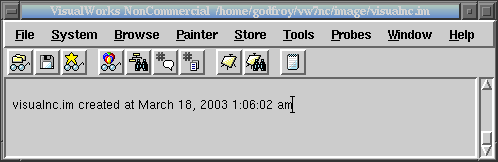
\includegraphics[scale=0.5]{nlesson1Fig1.png}
\caption{The Launcher of VisualWorks.\label{fig:launcher}}
\end{center}
\end{figure}}


This expression first creates a new instance of
\ct{SimpleCounter}, and then sends the message
\ct{value} to it and retrieve the current value of
\ct{value}. This should return nil (the default value
for noninitialised instance variables; afterwards we will create
instances where \ct{value} has a reasonable default
initialisation value). 


\exercise  Another method that is normally used besides the
accessor method is a so-called mutator method. Such a
method is used to change the value of an instance variable from a
client. For example, the next expression first create a new
\ct{SimpleCounter} instance and then sets the value of
\ct{value} to 7: \ct{SimpleCounter new value: 7}


This mutator method does not currently exist, so as an exercise
write the method \ct{value:} such that, when invoked on
an instance of \ct{SimpleCouter}, the \ct{value}
instance variable is set to the argument given to the message.
Test your method by typing and evaluating the expression above.

\exercise Implement the following methods in the protocol operations.

\begin{verbatim}
increment
    self value: self value + 1
decrement
    self value: self value - 1
\end{verbatim}

\exercise Implement the following methods in the protocol printing
\begin{verbatim}
printOn: aStream
    super printOn: aStream.
    aStream nextPutAll: ' with value: ', 
    							self  value printString.
    aStream cr.
\end{verbatim}

Now test the methods \ct{increment} and \ct{decrement} but pay attention that the counter value is not initialized. Try \ct{SimpleCounter new value: 0; increment ; value}.
Note that the method \ct{printOn:} is used when you print an
object or click on \ct{self} in an inspector. 

\subsection*{Adding an instance creation method}
When we create a new instance of the class \ct{SimpleCounter}
using the message \ct{new}, we would like to obtain a well
initialized instance. To do so, we need to override the method
\ct{new} to add a call to an initialization method (invoking
an \ct{initialize} method is a very common practice! Ask for
the senders of \ct{initialize}). Notice that \ct{new} is always
sent to a class. This means we have to define the new method on
the class side. To define an instance creation method like the
method \ct{new} you should be on the class side, so you click
on the \ct{Class} tab. 

\exercise Define a new protocol called \ct{instance creation},
and implement the method \ct{new} as follows:

\begin{code}
new
   "Create and return an initialized instance of SimpleCounter"
   |newInstance|
   newInstance := super new.
   newInstance initialize.
   ^ newInstance
\end{code}

This code returns a new and well initialized instance. We first
create a new instance by calling the normal creation method
(\ct{super new}), then we assign this new created instance
into the temporary variable called \ct{newInstance}. Then we
invoke the \ct{initialize} method on this new created instance
via the temporary variable and finally we return it.

Note that the previous method body is strictly equivalent to
the following one. Try to understand why they are equivalent.

\begin{code}
new
   "Create and return an initialized instance of SimpleCounter"

   ^ super new initialize
\end{code}

\subsection*{Adding an instance initialization method}
Now we have to write an initialization method that sets a default
value to the \ct{value} instance variable. However, as
we mentioned the \ct{initialize} message is sent to the newly
created instance. This means that the \ct{initialize} method
should be defined at the instance side as any method that is sent
to an instance of \ct{SimpleCounter} like \ct{increment}
and \ct{decrement}. The \ct{initialize} method does not
have specific and predefined semantics; it is just a convention to
name the method that is responsible to set up the instance
variable default values.

Therefore at the instance side, you should create a protocol
\texttt{initialize-release}, and create following method (the body
of this method is left blank. Fill it in!).

\begin{code}
initialize
   "set the initial value of the value to 0"
\end{code}

\paragraph{Remark.} As we already mentioned, the \ct{initialize} 
method is not automatically invoked by the method \ct{new}.
We had to override the method \ct{new} to call the
\ct{initialize} method. This is a weakness of the Smalltalk
libraries, so you should always check if the class that you are
creating inherits from a \ct{new} method that implements the
call to the \ct{initialize} method. It is a good practice to
add such a calling structure (\ct{new} calling
\ct{initialize}) in the root of the your class hierarchy. This
way you share the calling structure and are sure that the
\ct{initialize} method is always called for all your classes.

Now create a new instance of class \ct{SimpleCounter}. Is it
initialized by default? The following code should now work without
problem: \ct{SimpleCounter new increment}

\subsection*{Another instance creation method}
If you want to be sure that you have really understood the
distinction between instance and class methods, you should define
now a different instance creation method named
\ct{withValue:}. This method receives an integer as argument
and returns an instance of \ct{SimpleCounter} with the
specified value. The following expression should return 20.
\ct{(SimpleCounter withValue: 19) increment ; value}


\paragraph{A Difficult Point}
Let us just think a bit! To create a new instance we said that we
should send messages (like \ct{new} and \ct{basicNew}) to
a class. For example to create an instance of
\ct{SimpleCounter} we sent \ct{new} to
\ct{SimpleCounter}. As the classes are also objects in
Smalltalk, they are instances of other classes that define the
structure and the behavior of classes. One of the classes that
represents classes as objects is \ct{Behavior}. Browse the
class \ct{Behavior}. In particular, \ct{Behavior} defines
the methods \ct{new} and \ct{basicNew} that are
responsible of creating new instances. If you did not redefine the
new message locally to the class of \ct{SimpleCounter}, when
you send the message \ct{new} to the class
\texttt{SimpleCounter}, the new method executed is the one defined
in \ct{Behavior}.

\section*{SUnit}
Download the tutorial SUnit Explained from http://www.iam.unibe.ch/$\sim$ducasse/\-WebPages\-/Books.html and define a TestCase with several tests for the SimpleCounter class. To open the test runner execute \ct{TestRunner open}.

\section*{Saving your Work}
\storespecific{To save our work, simply publish your package. Saving the image is also one way to save your work but publishing it save the code in the database.}


\ifx\wholebook\relax\else\end{document}\fi

\ifx\wholebook\relax\else
\documentclass{report}
\usepackage{times}
\usepackage{epsfig}
\usepackage{alltt}
\usepackage{xspace}
\usepackage{graphicx}
\usepackage{ifpdf}
\usepackage{ifthen}
\usepackage{amsmath}
\usepackage{a4wide}

\graphicspath{{figures/}} 

\ifpdf
\DeclareGraphicsExtensions{.pdf, .jpg, .tif, .png}
\else
\DeclareGraphicsExtensions{.eps, .jpg}
\fi

\newboolean{toseecomment}
\setboolean{toseecomment}{false}
%%change to false to hidde comment 
\newcommand{\comment}[1]{\ifthenelse{\boolean{toseecomment}}{$\blacktriangleright$ \textit{#1}$\blacktriangleleft$}{}}

\newcommand{\commented}[1]{}

\newboolean{seevwspecific}
\setboolean{seevwspecific}{true}
\newcommand{\vwspecific}[1]{\ifthenelse{\boolean{seevwspecific}}{#1}{}}

\newboolean{seecategoryspecific}
\setboolean{seecategoryspecific}{false}
\newcommand{\categoryspecific}[1]{\ifthenelse{\boolean{seecategoryspecific}}{#1}{}}

\newboolean{seestorespecific}
\setboolean{seestorespecific}{true}
\newcommand{\storespecific}[1]{\ifthenelse{\boolean{seestorespecific}}{#1}{}}

\newboolean{seesqueakspecific}
\setboolean{seesqueakspecific}{false}
\newcommand{\squeakspecific}[1]{\ifthenelse{\boolean{seesqueakspecific}}{#1}{}}


\newcommand{\category}[0]
{\ifthenelse{\boolean{seestorespecific}}
	{package\xspace}
	{category\xspace}}

\newcommand{\ct}[1]{\texttt{#1}\xspace}
\newcommand{\stc}[1]{{\small {\sf #1}}\xspace}
\newcommand{\ST}{{\textsc Smalltalk}\xspace}
\newcommand{\tab}{\makebox[4em]{}}
\newcommand{\ttt}[1]{{\tt #1}}
\newcommand{\chev}{\ttt{>>}}
\newcommand{\vw}{VisualWorks\xspace}
\newcommand{\sq}{Squeak\xspace}
\newcommand{\store}{Store\xspace}
\renewcommand{\chaptername}{Exercise}
\newcommand{\exercise}{\vspace{0.2cm}\noindent \textbf{Exercise:}\xspace}

\newsavebox{\fminibox}
\newlength{\fminilength}

% Fait un truc encadre
\newenvironment{fminipage}[1][\linewidth]
  {\setlength{\fminilength}{#1-2\fboxsep-2\fboxrule}
        \begin{lrbox}{\fminibox}\begin{minipage}{\fminilength}}
  { \end{minipage}\end{lrbox}\noindent\fbox{\usebox{\fminibox}}}

% Pareil mais pas encadre (a utiliser pour ne pas couper une fonction

\newenvironment{nminipage}[1][\linewidth]
  {\setlength{\fminilength}{#1}
        \begin{lrbox}{\fminibox}\begin{minipage}{\fminilength}}
  { \end{minipage}\end{lrbox}\noindent\mbox{\usebox{\fminibox}}}

% Un alltt encadre
\newenvironment{falltt}
  {\vspace*{0.3cm}\begin{fminipage}\begin{alltt}}
  {\end{alltt}\end{fminipage}\vspace*{0.3cm}}

% Un alltt pas encadre
\newenvironment{nalltt}
  {\vspace*{0.3cm}\begin{nminipage}\begin{alltt}}
  {\end{alltt}\end{nminipage}\vspace*{0.3cm}}

% Une fonction encadree
\newenvironment{ffonction}[1]
  {\begin{fonction}[#1]
        \begin{fminipage}
\begin{alltt}
\rule{\linewidth}{0.5pt}}
{\end{alltt}\end{fminipage}\end{fonction}}

\newenvironment{codeonepage}
  {\begin{nminipage}\vspace*{0.2cm}\hrule\vspace*{0.1cm}
\begin{alltt}}
  {\end{alltt} \vspace*{-0.2cm}\hrule \vspace*{0.2cm} \end{nminipage}}

\newenvironment{code}
  {\vspace*{0.1cm}\hrule\vspace*{-0.1cm}\begin{alltt}}
  {\end{alltt}\vspace*{-0.2cm}\hrule \vspace*{0.1cm}}


\begin{document}
\fi

\chapter{A Simple Application: A LAN simulation}
\section*{Basic LAN Application }

The purpose of this exercise is to create a basis for writing
future OO programs. We use the knowledge of the previous
exercise to create classes and methods. We work on an
application that simulates a simple \textbf{Local Area Network (LAN)}.  We will
create several classes: \ct{Packet, Node, Workstation}, and
\ct{PrintServer}. We start with the simplest version of a LAN,
then we will add new requirements and modify the proposed
implementation to take them into account.

\subsection*{Creating the Class \ct{Node}}

The class \ct{Node} will be the root of all the entities that
form a \ct{LAN}. This class contains the common behavior
for all nodes. As a network is defined as a linked list
of nodes, a Node should always know its next node. A node should be
uniquely identifiable with a name. We represent the name of a node
using a symbol (because symbols are unique in Smalltalk) and the
next node using a node object. It is the node responsibility to
send and receive packets of information.

\begin{code}
Node inherits from Object
Collaborators: Node and Packet
Responsibility:
name (aSymbol) - returns the name of the node.
hasNextNode - tells if a node has a next node.
accept: aPacket - receives a packet and process it.
By default it is sent to the next node.
send: aPacket - sends a packet to the next node.
\end{code}


\exercise  Create a new \category \ct{LAN}, and create a
subclass of \ct{Object} called \ct{Node}, with two instance
variables: \ct{name} and \ct{nextNode}.

\exercise  Create accessors and mutators for the two instance
variables. Document the mutators to inform users that the argument
passed to \ct{name:} should be a Symbol, and the arguments
passed to \ct{nextNode} should be a Node. Define them in a
\ct{private} protocol. Note that a node is identifiable via
its name. Its name is part of its public interface, so you should
move the method name from the \ct{private} protocol to the
\ct{accessing} protocol (by drag'n'drop). \\

\exercise  Define a method called \ct{hasNextNode} that
returns whether the node has a next node or not. \\

\exercise  Create an instance method \ct{printOn:} that puts
the class name and name variable on the argument
\ct{aStream}. Include my next node's name ONLY if there is a
next node (Hint: look at the method \ct{printOn:} from
previous exercises or other classes in the system, and consider that the instance variable
\ct{name} is a symbol and \ct{nextNode} is a node). The expected \ct{printOn:} method behavior is described by the following code:

\begin{code}
(Node new
   name: \#Node1 ;
   nextNode: (Node new name: \#PC1)) printString

Node named: Node1 connected to: PC1
\end{code}

\exercise  Create a \textbf{class} method \ct{new} and an
\textbf{instance} method \ct{initialize}. Make sure that a new
instance of \ct{Node} created with the new method uses
\ct{initialize} (see previous exercise). Leave
\ct{initialize} empty for now (it is difficult to give meaningful
default values for the \ct{name} and \ct{nextNode} of
\ct{Node}. However, subclasses may want to override this
method to do something meaningful).

\exercise  A node has two basic messages to send and receive
packets. When a packet is sent to a node, the node has to accept
the packet, and send it on. Note that with this simple behavior
the packet can loop infinitely in the LAN. We will propose some
solutions to this issue later. To
implement this behavior, you should add a protocol
\ct{send-receive}, and implement the following two methods -in
this case, we provide some partial code that you should complete
in your implementation:

\begin{code}
accept: thePacket
 "Having received the packet, send it on. This is the default
behavior My subclasses will probably override me to do
something special"\\
    \dots

send: aPacket
"Precondition: self have a nextNode"

"Display debug information in the Transcript, then
send a packet to my following node"

 Transcript show:
   self name printString,
      ' sends a packet to ',
      self nextNode name printString; cr.
\dots
\end{code}

\begin{figure}[htbp]
\begin{center}
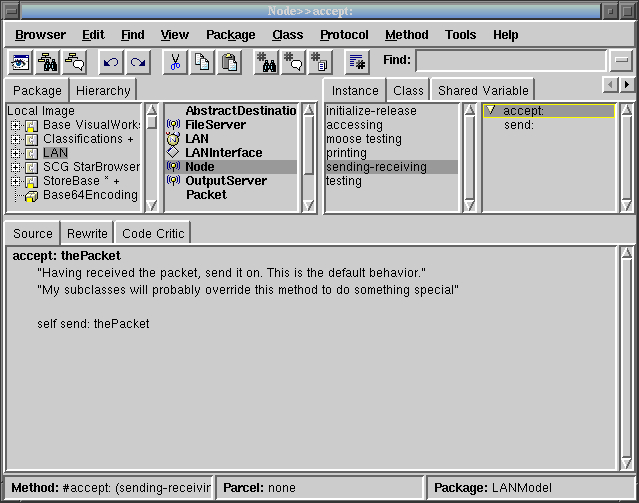
\includegraphics[scale=0.5]{nlesson3Fig1.png}
\caption{Definition of \ct{accept:} method}
\end{center}
\end{figure}



\subsection*{Creating the Class \ct{Packet}}

A packet is an object that represents a piece of information that is sent from node to node. So the responsibilities of this object are to allow us to define the originator of the sending, the address of the receiver and the contents.

\begin{code}
Packet inherits from Object
Collaborators: Node
Responsibility:
addressee returns the addressee of the node to which
the packet is sent.
contents - describes the contents of the message sent.
originator - references the node that sent the packet.
\end{code}

\exercise  In the \ct{LAN}, create a subclass of \ct{Object}
called \ct{Packet}, with three instance variables: \ct{contents},
\ct{addressee}, and \ct{originator}. Create accessors and mutators
for each of them in the \ct{accessing} protocol (in that
particular case the accessors represents the public interface of
the object). The addressee is represented as a symbol, the
contents as a string and the originator has a reference to a node.

\exercise  Define the method \ct{printOn: aStream} that puts a
textual representation of a packet on its argument
\ct{aStream}.

\subsection*{Creating the Class \ct{Workstation}}

A workstation is the entry point for new packets onto the LAN
network. It can originate packet to other workstations, printers
or file servers. Since it is kind of network node, but provides
additional behavior, we will make it a subclass of \ct{Node}.
Thus, it inherits the instance variables and methods defined in
\ct{Node}. Moreover, a workstation has to process packets
that are addressed to it.

\begin{code}
Workstation inherits from Node
Collaborators: Node, Workstation
and Packet
Responsibility: (the ones of node)
originate: aPacket - sends a packet.
accept: aPacket - perform an action on packets sent to the
workstation (printing in the transcript). For the other
packets just send them to the following nodes.
\end{code}

\exercise In the \category \ct{LAN} create a subclass of
\ct{Node }called \ct{Workstation} without instance
variables. \\

\exercise  Define the method \ct{accept: aPacket} so that if
the workstation is the destination of the packet, the following
message is written into the Transcript. Note that if the packets
are not addressed to the workstation they are sent to the next
node of the current one.

\begin{code}
(Workstation new
    name: \#Mac ;
    nextNode: (Printer new name: \#PC1))
          accept: (Packet new addressee: \#Mac)

A packet is accepted by the Workstation Mac
\end{code}

\textbf{Hints:} To implement the acceptance of a packet not addressed
to the workstation, you could copy and paste the code of the
\ct{Node} class. However this is a bad practice, decreasing
the reuse of code and the ``Say it only once'' rules. It is better
to invoke the default code that is currently overriden by using
\ct{super}.

\exercise  Write the body for the method \ct{originate:} that
is responsible for inserting packets in the network in the method
protocol \ct{send-receive}. In particular a packet should be
marked with its originator and then sent.

\begin{code}
originate: aPacket
 "This is how packets get inserted into the network.
  This is a likely method to be rewritten to permit
  packets to be entered in various ways. Currently,
  I assume that someone else creates the packet and
  passes it to me as an argument."
 \ldots

\end{code}

\subsection*{Creating the class \ct{LANPrinter}}

\exercise With nodes and workstations, we provide only limited
functionality of a real LAN. Of course, we would like to do
something with the packets that are travelling around the LAN.
Therefore, you will now create a class \ct{LanPrinter}, a special
node that receives packets addressed to it and prints them (on the
Transcript). Note that we use the name LanPrinter to avoid confusion with the existing class
\ct{Printer} in the namespace Smalltalk.Graphics (so you could use the name Printer in your namespace or the Smalltalk namespace if you really wanted to). Implement the class LanPrinter.

\begin{code}
LanPrinter inherits from Node
Collaborators: Node and Packet
Responsibility:
accept: aPacket - if the packet is addressed to the
printer, prints the packet contents else sends the packet
to the following node.
print: aPacket - prints the contents of the packet
(into the Transcript for example).
\end{code}


\subsection*{Simulating the LAN}

Implement the following two methods on the class side of the class
\ct{Node}, in a protocol called \ct{examples}. But take
care: the code presented below has \textbf{some bugs} that you should
find and fix!.

\begin{code}
simpleLan
  "Create a simple lan"
  "self simpleLan"

 | mac pc node1 node2 igPrinter |

"create the nodes, workstations, printers and fileserver"
mac := Workstation new name: \#mac.
pc := Workstation new name: \#pc.
node1 := Node new name: \#node1.
node2 := Node new name: \#node2.
node3 := Node new name: \#node3.
igPrinter := Printer new name: \#IGPrinter.

"connect the different nodes."
"I make following connections:
\tab \tab mac -\ct{>} node1 -\ct{>} node2 -\ct{>}
\tab \tab igPrinter -\ct{>} node3 -\ct{>} pc -\ct{>} mac"
mac nextNode: node1.
node1 nextNode: node2.
node2 nextNode: igPrinter.
igPrinter nextNode: node3.
node3 nextNode: pc.
pc nextNode: mac.

"create a packet and start simulation"
packet := Packet new
            addressee: \#IGPrinter;
            contents: 'This packet travelled around
to the printer IGPrinter.

mac originate: packet.
\end{code}

\begin{code}
\textbf{anotherSimpleLan}

"create the nodes, workstations and printers"

{\textbar}mac pc node1 node2 igPrinter node3 packet {\textbar}
mac:= Workstation new name: \#mac.

pc := Workstation new name:\#pc.

node1 := Node new name: \#node1.

node2 := Node new name: \#node2.

node3 := Node new name: \#node3.

igPrinter := LanPrinter new name: \#IGPrinter.

"connect the different nodes." "I make the following connections:
\tab \tab mac -\ct{>} node1 -\ct{>} node2 -\ct{>} \tab
\tab igPrinter -\ct{>} node3 -\ct{>} pc -\ct{>} mac"
mac nextNode: node1.

node1 nextNode: node2.

node2 nextNode:igPrinter.

igPrinter nextNode: node3.

node3 nextNode: pc.

pc nextNode: mac.

"create a packet and start simulation''
packet := Packet new
             addressee: \#anotherPrinter;
             contents: 'This packet travels around
             to the printer IGPrinter'.
pc originate: packet.
\end{code}


As you will notice the system does not handle loops, so we will
propose a solution to this problem in the future. To break the
loop, use either \textbf{Ctrl-Y} or \textbf{Ctrl-C}, depending on your VisualWorks version.

\subsection*{Creating the Class \ct{FileServer}}

Create the class \ct{FileServer}, which is a special node that
saves packets that are addressed to it (You should just display a
message on the Transcript).


\begin{code}
FileServer inherits from Node
Collaborators: Node and Packet
Responsibility:
accept: aPacket - if the packet is addressed to the
file server save it (Transcript trace) else send the
packet to the following node.
save: aPacket - save a packet.
\end{code}

\ifx\wholebook\relax\else\end{document}\fi

%\chapter{Fundamentals on the Semantics of Self and Super}


This lesson wants you to give a better understanding of self 
and super. 

\section{self}

When the following message is evaluated: 

\begin{code}
aWorkstation originate: aPacket
\end{code}

The system starts to look up the method originate: starts in 
the class of the message receiver: Workstation. Since this class 
defines a method originate:, the method lookup stops and this 
method is executed.

Following is the code for this method:

\begin{code}
Workstation\texttt{>>}originate: aPacket

   aPacket originator: self.
   self send: aPacket
\end{code}

\begin{enumerate}
    \item
It first sends the message originator: to an instance of Packet with 
as argument self which is a pseudo-variable that represents the 
receiver of originate: method. The same process occurs. Originator: 
is looked up into the class Packet. As Packet defines a method 
named originator:, the method lookup stops and the method is executed. 
As shown below the body of this method is to assign the value 
of the first argument (aNode) to the instance variable originator. 
Assignment is one of the few constructs of Smalltalk. It is not 
realized by a message sent but handle by the compiler. So no 
more message sends are performed for this part of originator:.

\begin{code}
Packet\texttt{>>}originator: aNode

      originator := aNode
\end{code}

\item
In the second line of the method originate:, the message send: 
thePacket is sent to self. self represents the instance that receives 
the originate: message. \textbf{The semantics of self specifies that 
the method lookup should start in the class of the message receiver.} 
Here Workstation. Since there is no method send: defined on the 
class Workstation, the method lookup continues in the superclass 
of Workstation: Node. Node implements send\textit{:}, so the method 
lookup stops and send: is invoked

\end{enumerate}

\begin{code}
 Node\texttt{>}\texttt{>}send: thePacket

      self nextNode accept: thePacket
\end{code}

The same process occurs for the expressions contained into the 
body of the method send:. 



\section{super}


Now we present the difference between the use of self and super. 
Self and super are both pseudo-variables that are managed by 
the system (compiler). They both represents the receiver of the 
message being executed. However, there is no use to pass super 
as method argument, self is enough for this.

The main difference between self and super is their semantics 
regarding method lookup. 

\begin{itemize}
\item
The semantics of self is to start the method lookup \textbf{into 
the class of the message receiver and to continue in its superclasses.}\\
\item
The semantics of super is to start the method look into \textbf{the 
superclass of class} \textbf{in which the method being executed was 
defined and to continue in its superclasses.}. Take care the semantics 
is \textbf{NOT} to start the method lookup into the superclass of 
the receiver class, the system would loop with such a definition 
(see exercise 1 to be convinced). Using super to invoke a method 
allows one to invoke overridden method.
\end{itemize}

Let us illustrate with the following expression: the message accept: 
is sent to an instance of Workstation. 

\begin{code}
aWorkstation accept: (Packet new addressee: \#Mac)
\end{code}

As explained before the method is looked up into the class of 
the receiver, here Workstation. The method being defined into 
this class, the method lookup stops and the method is executed. 

\begin{code}
 Workstation\texttt{>>}accept: aPacket

     (aPacket addressee = self name)
         ifTrue:\ensuremath{[}Transcript show: 'Packet accepted', self name asString\ensuremath{]}
         ifFalse: \ensuremath{[}super accept: aPacket\ensuremath{]}
\end{code}

Imagine that the test evaluates to false. The following expression 
is then evaluated.

\begin{code}
 super accept: aPacket
 \end{code}


The method accept: is looked up in the superclass of the class 
in which the containing method accept: is defined. Here the containing 
method is defined into Workstation so the lookup starts in the 
superclass of Workstation: Node. The following code is executed 
following the rule explained before. 

\begin{code}
Node\texttt{>>}accept: aPacket

     self hasNextNode\
         ifTrue:\ensuremath{[} self send: aPacket\ensuremath{]}
\end{code}

\textbf{Remark.} The previous example does not show well the vicious 
point in the super semantics: the method look into \textbf{the superclass 
of class} \textbf{in which the method being executed was defined and 
not in the superclass of the receiver class.}

You have to do the following exercise to prove yourself that 
you understand well the nuance.\\
\exercise 1: Imagine now that we define a subclass of Workstation 
called AnotherWorkstation and that this class does NOT defined 
a method accept:. Evaluate the following expression with both 
semantics:

\begin{code}
 anAnotherWorkstation accept: (Packet new addressee: \#Mac)
\end{code}

You should be convinced that the semantics of super change the 
lookup of the method so that the lookup (for the method via super) 
does NOT start in the superclass of the receiver class but in 
the superclass of the class in which the method containing the 
super. With the wrong semantics the system should loop.








\endinput
%\chapter{ Object Responsibility and Better Encapsulation}

\section{Reducing the coupling between classes }


To be a good citizen you as an object should follow as much as 
possible the following rules:

\begin{itemize}
\item
Be private. Never let somebody else play with your data.
\item
Be lazy. Let do other objects your job.
\item
Be focused. Do only one main task. 
\end{itemize}

While these guidelines are not really formal, one of the main 
consequences is that this is the responsibility of an object 
to provide a well defined interface protecting itself from its 
clients. The other consequence is that by delegating to other 
objects an object concentrates on a single task and responsibility. 
We now look how such guidelines can help us to provide better 
objects in our example.



\subsection{Current situation}


The interface of the packet class is really weak. It just provides 
free access to its data. The main impact of this weakness is 
the fact that the clients of the class Packet like Workstation relies 
on the internal coding of the Packet as shown in the first line 
of the following method.

\begin{code}
 Workstation\texttt{>>}accept: aPacket

    aPacket addressee = self name
       ifTrue:\ensuremath{[} Transcript show: 'A packet is accepted by the 
Workstation ', self name asString\ensuremath{]}
       ifFalse: \ensuremath{[}super accept: aPacket\ensuremath{]}
\end{code}


As a consequence, if the structure of the class Packet would 
change, the code of its clients would have to change too. Generalizing 
such a bad practice would lead to system that are badly coupled 
and being really difficult to change to meet new requirements.



\subsection{Solution.}

This is the responsibility of a packet to say if the packet is 
addressed to a particular node or if it was sent by a particular 
node.
\begin{itemize}
\item Define a method named isAddressedTo: aNode in `testing' protocol 
that answers if a given packet is addressed to the specified 
node. 
\item Define a method named isOriginatedFrom: aNode in `testing' protocol 
that answers if a given packet is originated from the specified 
node. 
\end{itemize}
Once these methods are defined, change the code of all the clients 
of the class Packet to call them.




\section{A Question of Creation Responsibility}


One of the problem with the previous approach for creating the 
nodes and the packets is the following:

it is the responsibility of the client of the objects to create 
them well-formed. For example, it is possible to create a node 
without specifying a name! This is a disaster for our LAN system 
(create an example method 3, and try it out). The same problem 
occurs with the packet: it is possible to create a packet without 
address nor contents.

We will find a solution to these problems.

\exercise  Define a class method named withName: in the class Node 
(protocol `instance creation') that creates a new node and assign 
its name.

\begin{code}
withName: aSymbol
....

\end{code}

Define a class method named withName:nextNode: in the class Node 
(protocol `instance creation') that creates a new node and assign 
its name and the next node in the LAN

\begin{code}
withName: aSymbol nextNode: aNode
....
\end{code}

Note that the first method can simply invoke the second one.

Define a class method named send:to\textit{:} in the class Packet (protocol `instance 
creation') that creates a new Packet with a contents and an address. 

\begin{code}
send: aString to: aSymbol\\
....
\end{code}

Now the problem is that we want to forbid the creation of non-well 
formed instances of these classes. To do so, we will simply redefine 
the creation method \textit{new} so that it will raise an error.

\exercise  Rewrite the new method of the class Node and Packet as 
the following:

\begin{code}
new

    self error: `you should invoke the method... to create a...' 
\end{code}

However, you have just introduced a problem: the instance creation 
methods you just wrote in exercise 11 will not work anymore, 
because they call \textit{new}, and that calling results in an error 
! The solution is to rewrite them such as 

\begin{code}
Node class\texttt{>>}withName: aSymbol nextNode: aNode
      ^ self basicNew initialize name: aSymbol ; nextNode: aNode
\end{code}

Do the same for the instance creation methods in class Packet.

\exercise Update and rerun your examples to make sure that 
your changes were correct.


Note that the previous code may break if a subclass specialize the nextNode: method
does not return the instance. To protect ourslef from possible unexpected
extension we add yourself that returns the receiver a the first cascaded message
(here name:), here the newly created instance. 

\begin{code}
Node class\texttt{>>}withName: aSymbol nextNode: aNode
      ^ self basicNew initialize name: aSymbol ; nextNode: aNode ; yourself
\end{code}


\section{Reducing the coupling between classes}


To be a good citizen you as an object should follow as much as 
possible the following rules:

\begin{itemize}
\item
Be private. Never let somebody else play with your private data.
\item
Be lazy. Let do other objects your job.
\item
Be focused. Do only one main task. 
\end{itemize}

While these guidelines are not really formal, one of the main 
consequences is that this is the responsibility of an object 
to provide a well defined interface protecting itself from its 
clients. The other consequence is that by delegating to other 
objects an object concentrates on a single task and responsibility. 
We now look how such guidelines can help us to provide better 
objects in our example.



\subsection{Current situation}

The interface of the packet class is really weak. It just provides 
free access to its data. The main impact of this weakness is 
the fact that the clients of the class Packet like Workstation relies 
on the internal coding of the Packet as shown in the first line 
of the following method.

\begin{code}
Workstation\texttt{>>}accept: aPacket

    aPacket addressee = self name\\
       ifTrue:\ensuremath{[} Transcript show: 'A packet is accepted by the Workstation ', self name asString\ensuremath{]}
       ifFalse: \ensuremath{[}super accept: aPacket\ensuremath{]}
\end{code}

As a consequence, if the structure of the class Packet would 
change, the code of its clients would have to change too. Generalizing 
such a bad practice would lead to system that are badly coupled 
and being really difficult to change to meet new requirements.



\subsection{Solution.}

This is the responsibility of a packet to say if the packet is 
addressed to a particular node or if it was sent by a particular 
node.

\begin{itemize}
\item Define a method named isAddressedTo: aNode in `testing' protocol 
that answers if a given packet is addressed to the specified 
node. 
\item Define a method named isOriginatedFrom: aNode in `testing' protocol 
that answers if a given packet is originated from the specified 
node. 
\end{itemize}


Once these methods are defined, change the code of all the clients 
of the class Packet to call them. You should note that a better 
interface encapsulates better the private data and the way they 
are represented. This allows one to locate the change in case 
of evolution.



\section{A Question of Creation Responsibility}


One of the problems with the first approach for creating the 
nodes and the packets is the following: it is the responsibility 
of the client of the objects to create them well-formed. For 
example, it is possible to create a node without specifying a 
name! This is a disaster for our LAN system, the node would never 
reachable, and worse the system would breaks because the assumptions 
that the name of a node is specified would not hold anymore (insert 
an anonymous node in Lan and try it out). The same problem occurs 
with the packet: it is possible to create a packet without address 
nor contents.

The solution to these problems is to give the responsibility 
to the objects to create well-formed instances. Several variations 
are possible:

\begin{itemize}
\item
When possible, providing default values for instance variable 
is a good way to provide well-defined instances.
\item
It is also a good solution to propose a consistent and well-defined 
creation interface. For example one can only provide an instance 
creation method that requires the mandatory value for the instance 
and forbid the creation of other instances.
\end{itemize}

\textbf{The class Packet.} 
We investigate the two solutions for the Packet class. For the 
first solution, the principle is that the creation method (new) 
should invoke an initialize method. Implement this solution. 
Just remember that new is sent to classes (a class method) and 
that initialize is sent to instances (instance method). Implement 
the method new in a `instance creation' protocol and initialize 
in a `initialize-release' protocol.

\begin{code}
Packet class\texttt{>>}new

\dots 

Packet\texttt{>>}initialize
   \dots 
\end{code}

The only default value that can have a default value is contents, 
choose 

\begin{code}
contents = `no contents'
\end{code} 


Ideally if each LAN would contain a default trash node, the default 
address and originator would point to it. We will implement this 
functionality in a future lesson. Implement first your own solution. 


\paragraph{Remarks and Analysis.} Note that with this solution it would 
be convenient to know if a packet contents is the default one 
or not. For this purpose you could provide the method hasDefaultContents 
that tests that. You can implement it in a clever way as shown 
below:

Instead of writing:

\begin{code}
Packet\texttt{>>}hasDefaultContents
 
 ^ contents = `no contents'

Packet\texttt{>>}initialize
 \dots 

contents := `no contents'
\dots 
\end{code}

You should apply the rule: `Say only once' and define a new method 
that returns the default content and use it as shown below:

\begin{code}
Packet\texttt{>>}defaultContents

    ^ `no contents'

Packet\texttt{>>}initialize
    \dots 

    contents := self defaultContent
    \dots 

Packet\texttt{>>}hasDefaultContent
    ^contents = self defaultContents
\end{code}

With this solution, we limit the knowledge to the internal coding 
of the default contents value to only one method. This way changing 
it does not affect the clients nor the other part of the class. 




\section{Proposing a creational interface}


\paragraph{Packet.}
We now apply the second approach by providing a better interface 
for creating packet. For this purpose we define a new creation 
method that requires a contents and an address.

Define a \textbf{class} methods named send:to\textit{:} and to: in the class Packet 
(protocol `instance creation') that creates a new Packet with a 
contents and an address. 

\begin{code}
Packet class\texttt{>>}send: aString to: aSymbol

....

Packet class\texttt{>>}to: aSymbol

....
\end{code}



\paragraph{The class Node.}

Now apply the same techniques to the class Node. Note that you 
already implemented a similar schema that the default value in 
the previous lessons. Indeed by default instance variable value 
is nil and you already implemented the method hasNextNode that 
to provide a good interface. \\
Define a \textbf{class} method named withName: in the class Node (protocol 
`instance creation') that creates a new node and assign its name.

\begin{code}
Node class\texttt{>>}withName: aSymbol

....
\end{code}

Define a \textbf{class} method named withName:connectedTo: in the class Node 
(protocol `instance creation') that creates a new node and assign 
its name and the next node in the LAN.

\begin{code}
 Node class\texttt{>>}withName: aSymbol connectedTo: aNode

....
\end{code}

Note that if to avoid to duplicate information, the first method 
can simply invoke the second one.



\section{Forbidding the Basic Instance Creation}


One the last question that should be discussed is the following 
one: should we or not let a client create an instance without 
using the constrained interface? There is no general answer, 
it really depends on what we want to express. Sometimes it could 
be convenient to create an uncompleted instance for debugging 
or user interface interaction purpose. 

Let us imagine that we want to ensure that no instance can be 
created without calling the methods we specified. We simply redefine 
the creation method new so that it will raise an error.

Rewrite the new method of the class Node and Packet as the following:

\begin{code}
Node class\texttt{>>}new

\tab \tab self error: `you should invoke the method... to create a...' 
\end{code}

However, you have just introduced a problem: the instance creation 
methods you just wrote in the previous exercise will not work 
anymore, because they call new, and that calling results in an 
error! Propose a solution to this problem.



\subsection{ Remarks and Analysis.}


A first solution could be the following code: 

\begin{code}
 Node class\texttt{>>}withName: aSymbol connectedTo: aNode

      ^ super new initialize name: aSymbol ; nextNode: aNode
\end{code}

However, even if the semantics permits such a call using super 
with a different method selector than the containing method one, 
it is a bad practice. In fact it implies an implicit dependency 
between two different methods in different classes, whereas the 
super normal use links two methods with the same name in two 
different classes. It is always a good practice to invoke the 
own methods of an object by using self. This conceptually avoids 
to link the class and its superclass and we can continue to consider 
the class as self contained.

The solution is to rewrite the method such as:

\begin{code}
Node class\texttt{>>}withName: aSymbol connectedTo: aNode

 ^  self basicNew initialize name: aSymbol ; nextNode: aNode
\end{code}

In Smalltalk there is a convention that all the methods starting 
with `basic' should not be overridden. basicNew is the method 
responsible for always providing an newly created instance. You 
can for example browse all the methods starting with `basic*' 
and limit yourself to Object and Behavior.

You can do the same for the instance creation methods in class Packet.



\section{Protecting yourself from your children}


The following code is a possible way to define an instance creation 
method for the class Node.

\begin{code}
Node class\texttt{>>}withName: aSymbol

 ^ self new name: aSymbol 
\end{code}

We create a new instance by invoking new, we assign the name 
of the node and then we return it. One possible problem with 
such a code is that a subclass of the class Node may redefine 
the method name: (for example to have a persistent object) and 
return another value than the receiver (here the newly created 
instance). In such a case invoking the method withName: on such 
a class would not return the new instance. One way to solve this 
problem is the following:


\begin{code}
Node class\texttt{>>}withName: aSymbol

 \ttt{|}newInstance\ttt{|}
 newInstance := self new.
 NewInstance name: aSymbol.
 ^ newInstance
\end{code}


This is a good solution but it is a bit too much verbose. It 
introduces extra complexity by the the extra temporary variable 
definition and assignment. A good Smalltalk solution for this 
problem is illustrated by the following code and relies on the 
use of the yourself message. 


\begin{code}
Node class\texttt{>>}withName: aSymbol

   ^ self new name: aSymbol ; yourself
\end{code}

yourself specifies that the receiver of the first message involved 
into the cascade (name: here and not new) is return. Guess what 
is the code of the yourself method is and check by looking in 
the library if your guess is right.





\endinput
%\chapter{ Hook and Template Methods}



\section{Providing Hook Methods}



\paragraph{Current situation. }


The solution proposed for printing a Node displays the following 
information: 

\begin{code}
(Node withName: \#Node1 connectedTo: (Node new name: \#PC1)) printString

      Node named: Node1 connected to: PC1
\end{code}

A straightforward way to implement the printOn: method on the 
class Node is the following code:

\begin{code}
Node\texttt{>>}printOn: aStream

 aStream nextPutAll: 'Node named: ', self name asString.
 self hasNextNode 
  ifTrue:\ensuremath{[} aStream nextPutAll: ' connected to: ', self nextNode name\ensuremath{]}
\end{code}

However, with such implementation the printing of all kinds of 
nodes is the same.



\paragraph{New Requirements.}
To help in the understanding of the LAN we would like that depending 
on the specific class of node we obtain a specific printing like 
the following ones:

\begin{code}
 (Workstation withName: \#Mac connectedTo: (LanPrinter withName: 
\#PC1) printString

   Workstation Mac connected to Printer PC1

(LanPrinter withName: \#Pr1 connectedTo: (Node withName: \#N1) 
printString

 Printer Pr1 connected to Node N1
\end{code}

Define the method typeName that returns a string representing 
the name of the type of node in the `printing' protocol. This 
method should be defined in Node and all its subclasses. 

\begin{code}
(LanPrinter withName: \#PC1) typeName

      `Printer'

(Node withName: \#N1) typeName
     `Node'
\end{code}

 
Define the method simplePrintString on the class Node to provide 
more information about a node as show below:

\begin{code}
(Workstation withName: \#Mac connectedTo: (LanPrinter withName: 
\#PC1)) simplePrint

`Workstation Mac'

(LanPrinter withName: \#PC1) simplePrint

`Printer PC1'
\end{code}

Then modify the printOn: method of the class Node to produce 
the following output:
\begin{code}
(self withName: \#Mac connectedTo: (LanPrinter new name: 
\#PC1))

`Node Mac connected to Printer PC1'
\end{code}

\paragraph{Remark:} The method typeName is called a \textit{hook} method. This 
reflects the fact that it allows the subclasses to specialize 
the behavior of the superclass, here the printing of a all the 
different kinds of nodes. The method simplePrintString, even 
if in our case is rather simple, is called a template method. 
This name reflects the fact that the method specifies the context 
in which hook methods will be called and how they will fit into 
the template method to produce the expected result. 


Note that for abstract classes hook methods can be abstract too, 
one other case the hook method can propose a default behavior.

The Smalltalk class library contains a lot of such hooks that 
allows an easy customization of the proposed behavior. The proposed 
requirement already exists in the system. Study the method printOn: 
on the class Object. 

\endinput
%\chapter{ Extending the LAN Application}


This lesson uses the basic LAN-example and adds new classes and 
behaviour. Doing so, the design is extended to be more general 
and adaptive.



\section{Handling Loops}


When a packet is sent to an unknown node, it loops endlessly 
around the LAN. You will implement two solutions for this problem. 

\paragraph{Solution 1.} The first obvious solution is to avoid that a node 
resends a packet if it was the originator of the packet that 
it is sent. Modify the accept: method of the class Node to implement 
such a functionality. 

\paragraph{Solution 2.} The first solution is fragile because it relies on 
the fact that a packet is marked by its originator and that this 
node belongs to the LAN. A `bad' node could pollute the network 
by originate packets with a anonymous name. Think about different 
solutions.

Among the possible solutions, two are worth to be further analyzed:
\begin{enumerate}
\item 
Each node keeps track of the packets it already received. When 
a packet already received is asked to be accepted again by the 
node, the packet is not sent again in the LAN. This solution 
implies that packet can be uniquely identified. Their current 
representation does not allow that. We could imagine to tag the 
packet with a unique generated identifier. Moreover, each node 
would have to remember the identity of all the packets and there 
is no simple way to know when the identity of treated node can 
be removed from the nodes.
\item 
Each packet keeps track of the node it visited. Every time a 
packet aarrived at a node, it is asked if it has already been 
here. This solution implies a modification of the communication 
between the nodes and the packet: the node must ask the status 
of the packet. This solution allows the construction of different 
packet semantics (one could imagine that packets are broadcasted 
to all the nodes, or have to be accepted twice). Moreover once 
a packet is accepted, the references to the visited nodes are 
simply destroyed with the packet so there is no need to propagate 
this information among the nodes. 
\end{enumerate}

We propose you to implement the second solution so that the class Packet 
provides the following interface (the new responsibilities are 
in bold).

\begin{code}
Packet inherits from Object\\
Collaborators: Node\\
Responsibility:\\
addressee returns the addressee of the node to which the packet 
is sent.\\
contents describes the contents of the message sent.\\
originator references the node that sent the packet.\\
isAddressedTo: aNode answers if a given packet is addressed to 
the specified node. isOriginatedFrom: aNode answers if a given 
packet is originated from the specified node. \\
\textbf{isAcceptableBy: aNode} answers if a packet is acceptable by 
a node\\
\textbf{hasBeenAcceptedBy: aNode} tells a packet that it has been 
accepted by a given node. \\
\end{code}

\begin{itemize}
\item
New instance variable. A packet needs to keep track of the nodes 
it visited. Add a new instance variable called visitedNodes in 
the class Packet. We want to collect the visited nodes in a set. Browse 
the class Set and its superclass to find the function you need.\\
\item
Initialize the new instance variable. Modify the initialize methods 
of the class Packet so that the visitedNodes instance variable 
is initialized with an empty set. \\
\item
Node Acceptation Methods. In a protocol named `node acceptation', 
define the method isAcceptableBy: and hasBeenAcceptedBy:. \\
\item
Test if your implementation works by sending a `bad' node with 
a bad originator into the LAN. 
\end{itemize}



\section{Introducing a Shared Initialization Process}


As you noticed, each time a new class is created that is not 
a subclass of Node we have to implement a new method whose the 
only purpose was to call the initialize method. We want to habe 
such a behavior specified only once and shared by all our Lan 
classes. 

Define a class LanObject that inherits form Object, implements 
an instance method initialize and a class method new that automatically 
calls the initialize method on the newly created object and retrun 
it. 

Then make all the classes that previously inherited from Object 
inherit from LanObject and check and remove if necessary if the 
unnecessary new methods. 



\section{Broadcasting and Multiple Addresses}

Up to now, when a packet reaches a node it is addressed to, the 
packet is handled by the node and the transmission of the packet 
is terminated (because is not sent to the next node in the network). 
In this exercise, we want you to provide facilities for broadcasting. 
If a node handles a packet that is broadcasted, the packet must 
be sent to the next node in the LAN instead of terminating the 
connection. For example, broadcasting makes it possible to save 
the contents of the same packet on different fileservers of the 
LAN. First try to solve this problem, and implement it afterwards.\\
 In the current LAN, a packet only has one addressee. This exercise 
wants to add packets that have multiple addressees. Propose a 
solution for this problem, and implement it afterwards.



\section{Different Documents}


Suppose we have several kinds of documents (ASCII and Postscript) 
and two kinds of LANPrinter in the LAN (LANASCIIPrinter and LANPostscriptPrinter). 
We then want to make sure that every printer prints the right 
kind of document. Propose a solution for this problem.



\section{Logging Node}

We want to add a logging facility: this means each time a packet 
is sent from a node, we want to identify the node and the packet. 
Propose and implement a solution. Hint: introduce a new subclass 
of Node between Node and its subclasses and specialize the send: 
method. 




\section{Automatic Naming }


The name of a node have to be specified by its creator. We would 
like to have an automatic naming process that occurs when no 
name are specified. Note that the names should be unique. As 
a solution we propose you to use a counter, as this counter have 
to last over instance creations but still does not have any meaning 
for a particular node we use an instance variable of the class 
node.

Note that the NetworkManager could also be the perfect object 
to implement such a fonctionality.
We also would like that all the printer names start with Pr. 
Propose a solution. 

\stc{ Workstation Mac connected to Printer PC}

\endinput
\appendix

\end{document}
